%
% teil1.tex -- Beispiel-File für das Paper
%
% (c) 2020 Prof Dr Andreas Müller, Hochschule Rapperswil
%
% !TEX root = ../../buch.tex
% !TEX encoding = UTF-8
%
\section{Mathematische Modellbildung
\label{openfoam:section:teil1}}
\kopfrechts{Mathematische Modellbildung}
Zum Simulieren von Strömungen benötigen wir zuerst ein Modell, das das Verhalten der Flüssigkeit möglichst umfassend und genau beschreibt. 
Hierbei werden meist die Navier-Stokes-Gleichungen benutzt, welche noch mit Randbedingungen und Zustandsgleichungen erweitert werden können. 
Oft werden aber auch die Euler-Gleichungen anstelle der Navier-Stokes-Gleichungen verwendet, da diese weniger Rechenaufwand benötigen,
\index{Navier-Stokes-Gleichung}%
dies aber auf Kosten der Genauigkeit.

Zudem benötigen wir ein Lösungsverfahren, das einen Anfangszustand und das mathematische Modell zu einer numerischen Lösung verarbeiten kann, dies ist nötig, da für die Navier-Stokes-Gleichungen keine analytische Lösung existiert.
Für die Euler-Gleichungen würden analytische Lösungen existieren, diese sind jedoch aufwändig zu berechnen.
\index{Euler-Gleichung}%
Deswegen werden auch zum Lösen der Euler-Gleichungen numerische Methoden verwendet.
Hierbei kommen meist die Finite-Differenzen-Methode (FDM), die Finite-Volumen-Methode (FVM) und die Finite-Elemente-Methode (FEM) zum Einsatz. 
\index{Finite-Differenzen-Methode}%
\index{FDM}%
\index{Finite-Volumen-Methode}%
\index{FVM}%
\index{Finite-Element-Methode}%
\index{FEM}%

\subsection{Stationär oder zeitabhängig?}
Bei der Strömungsmechanik wird zuerst unterschieden, ob es sich um eine stationäre oder zeitabhängige Strömung handelt.
\index{stationar@stationär}%
\index{zeitabhangig@zeitabhängig}%
Das heisst es ist entweder der Fall, dass an jedem Ort im Raum die Geschwindigkeit, der sich dort befindenden Flüssigkeit  konstant ist oder dass sich diese Grösse dauernd ändert.

Wenn die Resultate kaum mehr ändern, ist der stationäre Zustand erreicht und es können keine neuen Resultate mehr erwartet werden.
Dadurch kann man sich Simulationsaufwand sparen.

\subsection{Modellierung der Flüssigkeit}
Im Kontext der CFD-Simulation nimmt man an, dass eine Flüssigkeit nicht aus einzelnen Teilen wie Atomen oder Molekülen besteht, sondern man nimmt an, sie sei kontinuierlich. 
Ausserdem geht man davon aus, dass sämtliche Eigenschaften der Flüssigkeit stetig sind. 

Zudem hat eine Flüssigkeit noch weitere Eigenschaften wie die Dichte. 
Diese kann hier aber nicht immer als konstant angesehen werden, da man ansonsten bei kompressiblen Flüssigkeiten einen Teil der Energie, welcher für das Komprimieren derselben verwendet wird, nicht beachten würde.
\index{kompressibel}%
Dies wiederum würde im Fall, dass die Kompressibilität beachtet werden muss, zu Abweichungen zwischen Simulation und Realität führen.
Auch müssen die Viskosität und die spezifische Wärmekapazität beschrieben werden.
\index{Viskositat@Viskosität}%
\index{Warmekapazitat@Wärmekapazität}%

\subsection{Die Euler-Gleichungen}
Die Euler-Gleichungen beschreiben das Verhalten der Strömung eines reibungsfreien Fluids, also eines laminaren Flusses, dessen Reibung vernachlässigt werden kann. 
\index{laminar}%
Das bedeutet, sie können nicht für alle Probleme eingesetzt werden. 
Sobald Reibungskräfte einen substantiellen Einfluss auf die Strömung haben, weist das berechnete Ergebnis eine Abweichung zur Realität auf.

\subsubsection{Massenerhaltung}
Das Gesetz der Massenerhaltung beschreibt, dass sich die Masse in einem geschlossenen System nicht verändern kann, ohne dass man Masse hinzufügt oder entfernt. 
\index{Massenerhalt}%
Dieses Verhalten beschreibt die zweite Euler-Gleichung, indem die Veränderung der Masse durch den Fluss von Masse durch eine Systemgrenze beschrieben wird.

Die erste Euler-Gleichung geht aus der Idee hervor, dass man ein beliebiges Volumen $V$ hat, das fest im Raum liegt. Durch ein Oberflächenstück 
$d \mathbf{S} $ 
des Volumens 
$V$
 fliesst jeweils der Massenstrom 
$ \rho\mathbf{u}\cdot d\mathbf{S}$, wobei $\mathbf{u}$ die Geschwindigkeit des Massenstromes ist.
Aus dem Massenstrom des Oberflächensegments kann man dann mit dem Oberflächenintegral 
\[\int_{S}\rho\mathbf{u}\cdot d\mathbf{S}\]
den gesamten Massenstrom berechnen. Dieser Massenstrom muss nun gleich sein wie die Massenänderung 
\[\frac{\partial M}{\partial t}\]
der in dem Volumen enthaltenen Flüssigkeit.
Diese Massenänderung berechnet man ausgehend vom Integral zum Berechnen der Masse 
\[M 
= 
\int_{V} \rho \, dV\]
im Kontrollvolumen $V.$
Um die Massenänderung zu erhalten, leitet man dieses Integral partiell nach $t$ ab und erhält so
\[\frac{\partial M}{\partial t}
=
\frac{\partial }{\partial t} \int_{V}\rho dV.\]
Hier nimmt man die Ableitung auf der rechten Seite noch in das Integral hinein, da dies später das Rechnen erleichtert.

Setzt man nun die beiden Terme der Massenänderung gleich, erhält man die Gleichung 
\[\int_{S}\rho\mathbf{u}\cdot d\mathbf{S} 
=
\int_{V} \frac{\partial \rho}{\partial t} \, dV .\] 
Bei dieser Gleichung kann man nun auf der linken Seite mit dem gaussschen Integralsatz das Oberflächenintegral in ein Volumenintegral umwandeln, es wird also zu
\index{Integralsatz von Gauss}%
\index{gaussscher Integralsatz}%
\[\int_{V}\nabla\cdot(\rho\mathbf{u}) \, dV
=
\int_{V}\frac{\partial \rho}{\partial t}  \, dV .\]
Ändert man nun die Flussrichtung des Massenstromes, indem man das Vorzeichen der rechten Seite wechselt, lässt sich die Gleichung umstellen.
Man erhält so
\[\int_{V}\nabla\cdot(\rho\mathbf{u})  \, dV + \int_{V}\frac{\partial \rho}{\partial t}  \, dV 
= 
0.\] 
Davon ausgehend können die Integrale zu einem Integral
\[\int_{V} \frac{\partial \rho}{\partial t} + \nabla\cdot(\rho\mathbf{u})  \, dV 
= 
0\]
zusammengefasst werden.

Dies kann nun in einem letzten Schritt in die Differentialgleichung
\begin{equation}
\label{openfoam:euler1}
\frac{\partial \rho}{\partial t} + \nabla\cdot(\rho\mathbf{u})  \, dV 
= 
0
\end{equation}
umgewandelt werden.
Wieso dies möglich ist, wird im Lemma \ref{maxwell:lemma:ampere} erläutert.

\subsubsection{Impulserhaltung}
Die zweite Euler-Gleichung beschreibt das Gesetz der Impulserhaltung. 
\index{Impulserhaltung}%
Es besagt, dass der Gesamtimpuls eines mechanisch abgeschlossenen Systems konstant ist.
Dies wird beschrieben, indem man die Änderung des Impulses eines Systems auf null setzt.
Diese Impulsänderung besteht aus den aussen anliegenden Kräften und den Kräften, wie Schwerkraft, die auf das ganze System wirken.
Bei der Impulserhaltung geht man fast gleich vor wie beim Herleiten der Gleichung für die Massenerhaltung.
Man geht ebenfalls von einem beliebigen Volumen Flüssigkeit, $V$, aus.
Bei der Impulserhaltung ist dieses Volumen aber nicht mehr an einem festen Ort, sondern es bewegt sich durch den Raum.
Ausserdem ist der Masseninhalt nicht mehr beliebig, sondern das Volumen beinhaltet eine feste Menge Masse.

Dieses Volumen weist nun eine Impulsänderung die
\[\frac{D}{Dt}\int_{V}\rho\mathbf{u}\, dV\]
entspricht.
Hier wird nicht mehr die partielle Ableitung verwendet, da das Kontrollvolumen nicht an einem festen Ort ist.
Anstelle der partiellen Ableitung wird eine substantielle Ableitung \[\frac{D}{Dt}\] verwendet, da diese die Änderung des Feldes an einem bewegten Teilchen beschreibt.

Als nächstes berechnet man die gesamte Kraft auf die Oberfläche des
Volumens $V$, in dem man alle Kräfte $\mathbf{f} = \mathbf{t}\,dS$,
die auf die Oberflächenstücke $dS$ wirken, integriert.
$\mathbf{t}\, dS$ ist hier gleich $(\mathbf{n\cdot\sigma}dS)$.
Dabei ist $\sigma$ der Spannungstensor, welcher genutzt wird um die drei Spannungsvektoren zusammenzufassen.
\index{Spannungstensor}%
Der Spannungsvektor, der auf die Oberfläche mit Normalenrichtung $\mathbf{n}$ wirkt, ist das Produkt des Spannungstensors mit $\mathbf{n}$.
So erhält man die Kraft 
\[\mathbf{F} 
=
\int_{S}\mathbf{f}\, dS
= \int_{S} (\mathbf{\sigma}\cdot d\mathbf{S})
.\]
Dies ist nun wieder ein Flächenintegral, das mit dem gaussschen Integralsatz in ein Volumenintegral umgewandelt werden kann.
\index{gaussscher Integralsatz}%
\index{Integralsatz von Gauss}%
Dadurch ergibt sich
\[\mathbf{F} 
=
\int_{V}\nabla \cdot \mathbf{\sigma}\, dV
.\]

Zuletzt berechnen wir noch den Einfluss anderer Kräfte wie die Schwerkraft auf den Impuls des Volumens $V$.
Dazu integrieren wir die normalisierte Volumenkraft $\mathbf{b}$, über alle Volumenstücke $dV$ wodurch wir das Integral 
\[\mathbf{F} 
=
\int_{V}\rho\mathbf{b}\, dV
\]
erhalten.
Die normalisierte Volumenkraft ist dabei zum Beispiel die Schwerkraft, die das gesamte Volumen wirkt. 
Sie wird noch auf die Masse normalisiert, man erhält also eine Beschleunigung.

Nun können wir die Impulsänderung des Volumens gleich der Summe der darauf wirkenden Kräfte setzen und die Integrale in einem Integral zusammenfassen. Daraus erhalten wir mit der Bedingung, die Masse im Volumen sei konstant, die Gleichung 
\[\int_{V} \rho \frac{D\mathbf{u}}{Dt} - \nabla \cdot \mathbf{\sigma} -\rho \mathbf{b}\, dV
=
0.
\]
Das Integral kann man wie bei \eqref{openfoam:euler1} dank Lemma \ref{maxwell:lemma:ampere} weglassen, wodurch wir die Differentialgleichung
\begin{equation}
\label{openfoam:euler2_1}
\rho \frac{D\mathbf{u}}{Dt}
= 
\nabla \cdot \mathbf{\sigma} +\rho \mathbf{b}
\end{equation}
erhalten.

Zuletzt kann man noch die substantielle Ableitung in eine partielle Ableitung umwandeln, damit wir die gleiche Form wie für die Massenerhaltungsgleichung erhalten.
\index{substantielle Ableitung}%
Dazu nutzen wir die Definition der substantiellen Ableitung
\[
\frac{D\Phi(\mathbf{x},t)}{Dt}
:=
\frac{\partial \Phi}{\partial t}+(\mathbf{u}\cdot \nabla)\Phi
,\] 
die beschreibt, wie die substantielle Ableitung mit der partiellen zusammenhängt.
Eingesetzt in die Differentialgleichung erhalten wir so 
\begin{equation}
\label{openfoam:euler2}
\rho\frac{\partial\mathbf{u}}{\partial t} + \nabla \cdot(\rho\mathbf{u}\otimes \mathbf{u})
= 
\nabla \cdot \mathbf{\sigma} +\rho \mathbf{b}.
\end{equation}
Diese Form erleichtert die Berechnung, da sie nicht mehr die Impulsänderung einer sich bewegenden Menge Flüssigkeit beschreibt, sondern die Impulsänderung der sich momentan an einem Ort befindenden Masse. 
Man kann also anstelle ein sich durch den Raum bewegendes Masseteilchen ein festes Volumenelement simulieren, welches bei der Fluid-dynamik-Simulation die bevorzugte Methode ist.
Auch zu sehen ist hier das dyadische Produkt, das mit $\mathbf{u}\otimes \mathbf{u}$ gebildet wird.
\index{dyadisches Produkt}%
Es wird verwendet, um mit dem Term $\nabla \cdot(\rho\mathbf{u}\otimes \mathbf{u})$, eine Advektion zu beschreiben.
Das dyadische Produkt, auch Tensorprodukt genannt, beschreibt eine Matrix aller Komponenten der Vektoren miteinander multipliziert.
\index{Tensorprodukt}%
Wendet man es auf den Geschwindigkeitsvektor $\mathbf{u}$ an, erhält man
\begin{equation}
\mathbf{u}\otimes \mathbf{u}
= 
\begin{pmatrix}
	u_x u_x &  u_x u_y & u_x u_z \\
	u_y u_x &  u_y u_y & u_y u_z \\
	u_z u_x &  u_z u_y & u_z u_z \\
\end{pmatrix}
.
\end{equation}
Wenn man nun noch die Divergenz dieser Matrix berechnet, resultiert
\begin{equation}
\nabla \cdot 
\begin{pmatrix}
	u_x u_x &  u_x u_y & u_x u_z \\
	u_y u_x &  u_y u_y & u_y u_z \\
	u_z u_x &  u_z u_y & u_z u_z \\
\end{pmatrix}
= 
\renewcommand{\arraystretch}{1.9}
\begin{pmatrix}
\displaystyle
	\frac{\partial u_x u_x}{\partial x} +  \frac{\partial u_x u_y}{\partial y} + \frac{\partial u_x u_z}{\partial z} \\
\displaystyle
	\frac{\partial u_y u_x}{\partial x} +  \frac{\partial u_y u_y}{\partial y} + \frac{\partial u_y u_z}{\partial z} \\
\displaystyle
	\frac{\partial u_z u_x}{\partial x} +  \frac{\partial u_z u_y}{\partial y} + \frac{\partial u_z u_z}{\partial z}  \\
\end{pmatrix}
.
\end{equation}
\subsubsection{Energieerhaltung}
Die dritte der Euler-Gleichungen wurde nicht wie die der Masse- und Impulserhaltung von Leonhard Euler hergeleitet, sie wird jedoch auch als Euler-Gleichung bezeichnet.
\index{Euler, Leonhard}%

Das Gesetz der Energieerhaltung besagt, dass die gesamte Energie in einem isolierten System konstant bleibt.
\index{Energieerhaltung}%
Diese Energie setzt sich im Fall der Fluiddynamik aus kinetischer, potenzieller und thermischer Energie zusammen.
Sie wird durch mechanische Arbeit, die äussere Kräfte leisten, verändert. Ebenso können Wärmequellen den Wärmeinhalt beeinflussen.
\index{mechanische Arbeit}%
\index{Warmeinhalt@Wärmeinhalt}%
\index{Warmequellen@Wärmequellen}%

Um die Energieerhaltung zu beschreiben, muss also die Änderung der thermischen Energie $e$ und die der kinetischen Energie $K$ bestimmt werden.
\index{thermische Energie}%
\index{Energie!thermisch}%
\index{kinetische Energie}%
\index{Energie!mechanisch}%
Bei $e$ und  $K$ handelt es sich jeweils um eine spezifische, also auf die Masse normalisierte, Energie.
Deswegen wird im Term 
\[\rho \frac{De}{Dt}+  \rho \frac{DK}{Dt},
\]
der die totale Energieänderung beschreibt, die Energie jeweils mit der Dichte $\rho$ multipliziert.

Nun muss anhand des Zuflusses mechanischer und thermischer Energie die Änderung der totalen Energie bestimmt werden.
Dabei wird noch zwischen internen und externen Energiequellen unterschieden.
Total muss man also zwischen vier unterschiedlichen Quellen unterscheiden, die eine Änderung der Energie im Kontrollvolumen verursachen.
Die Änderung der thermischen Energie wird durch die Terme  $- \nabla \cdot \mathbf{q}$ und  $\rho r$ dargestellt, wobei der erste einen Zufluss durch die Oberfläche des Kontrollvolumens und der zweite eine Energiequelle im Inneren desselben beschreibt.
Dabei sind $\mathbf{q}$ und $r$ auf Fläche respektive Volumen normalisierte Wärmequellen.
Die mechanischen Energiequellen werden durch die Terme $\nabla \cdot (\sigma \cdot \mathbf{u})$ und $\rho \mathbf{b} \cdot \mathbf{u}$ beschrieben.
Hier handelt es sich beim ersten Term wieder um einen Zufluss an mechanischer Energie durch die Oberfläche des Kontrollvolumens.  Der zweite Term beschreibt hier aber die Änderung der potenziellen Energie aufgrund von Kräften, wie der Schwerkraft, die auf die gesamte Masse im Volumen wirken.
Aus allen diesen Termen zusammen lässt sich die Differentialgleichung
\begin{equation}
\label{openfoam:euler3}
\rho \frac{De}{Dt}+  \rho \frac{DK}{Dt}
=
- \nabla \cdot \mathbf{q} + \rho r + \nabla \cdot (\sigma \cdot \mathbf{u}) + \rho \mathbf{b} \cdot \mathbf{u} 
\end{equation} 
bilden.

\subsection{Die Navier-Stokes-Gleichungen}
Die Navier-Stokes-Gleichungen sind eine Erweiterung der Euler-Gleichungen, welche zusätzlich noch die Viskosität der Flüssigkeit berücksichtigen.
\index{Navier-Stokes-Gleichungen}%
Dadurch können Flüssigkeiten genauer modelliert werden als mit den Euler-Gleichungen, da in Fällen, in denen die Reibung der Flüssigkeit einen grossen Einfluss auf das Resultat hat, das Modell vollständiger ist.
\index{Viskositat@Viskosität}%
\index{Reibung}%

Die erste Gleichung, die wir benötigen, ist die Massenerhaltungs-Gleichung.
Diese haben wir schon in Gleichung \eqref{openfoam:euler1} erhalten.

Dazu kommt noch die Navier-Stokes-Impulserhaltungsgleichung.
Sie beschreibt die Veränderung des Impulses in einem Kontrollvolumen aufgrund innerer Kräfte durch einen Druckunterschied, Reibungskräfte durch Flüssigkeitsbewegung und Kräfte, die von aussen auf das ganze Volumen wirken.

Die Kräfte, die durch Druckunterschiede hervorgerufen werden, werden mit dem Term $- \nabla p$ beschrieben.
Man nimmt also die negative Divergenz des Druckfeldes um alle Kräfte, die von Gebieten mit höherem Druck zu Gebieten mit tieferem Druck zeigen, zu beschreiben.

Der nächste benötigte Term ist $\mu \Delta \mathbf{u}$, darin wird ein Impulstransport zwischen Schichten der Flüssigkeit mit unterschiedlicher Geschwindigkeit beschrieben.
Dazu nutzt man die kinematische Viskosität $\mu$, sie beschreibt wie viel Kraft benötigt wird, zwei Schichten einer Flüssigkeit aneinander vorbei zu bewegen.
\index{kinematische Viskositat@kinematische Viskosität}%
\index{Viskositat@Viskosität!kinematisch}%
Die zu überwindenden Kräfte entstehen dabei durch Intermolekulare Verbindungen wie die Van-der-Waals-Kräfte.
\index{Van-der-WaalsKrafte@Van-der-Waals-Kräfte}%
Der zweite Teil, $\Delta \mathbf{u}$, beschreibt wie sich ein Impuls in der Flüssigkeit ausgleicht.
Dazu wird der Laplace-Operator auf das Geschwindigkeitsfeld angewandt.

Den letzten Term den wir benötigen beschreibt die Impulsänderung aufgrund von Kräften, die auf das ganze Kontrollvolumen wirken.
Dieser Term, $\rho \mathbf{b}$, wird aus der Gleichung \eqref{openfoam:euler2} wiederverwendet.

Diese drei Terme zusammen beschreiben die Impulsänderung 
\begin{equation}
\rho \frac{D\mathbf{u}}{Dt}
=
- \nabla p + \mu \Delta \mathbf{u} +\rho \mathbf{b} 
.\end{equation}
Dadurch, dass diese Impulserhaltungsgleichung die Reibung der Flüssigkeit beachtet, eignet sie sich besser, um turbulente Flüssigkeiten zu simulieren. 

\subsection{Randbedingungen}
\label{openfoam:randbedingungen}
Mit den Randbedingungen definiert man, wie die Flüssigkeit mit dem Rand des Gebietes, auf welchem man das mathematische Modell der Flüssigkeit anwendet, interagiert.
Dabei kann man für verschiedene Gebiete des Randes jeweils unterschiedliche Bedingungen wählen, um zum Beispiel einen Fluss von einem Eingang durch das Volumen zu einem Ausgang zu beschreiben.

Zum Rand gehört die Begrenzung des Gebietes, auf das man das Modell der Flüssigkeit anwenden will, aber auch die Oberflächen der Objekte, die sich innerhalb dieses Gebietes befinden.
Den Raum zwischen dem äusseren Rand und dem Rand des Objektes nennt man Lösungs-Domain, in dieser Region befindet sich die Flüssigkeit, deren Verhalten man berechnen möchte.
\index{Losungs-Domain@Lösungs-Domain}%

\subsubsection{Inlet}
\index{Inlet}%
Im Falle eines Inlets wird auf einen Bereich des Randes ein fester Wert festgelegt. 
So werden zum Beispiel die Geschwindigkeit und Temperatur einer Region fest bestimmt.
Druck und Geschwindigkeit sind aber nicht unabhängig voneinander, daher muss der Druck frei belassen werden und es wird anstelle eines festen Wertes der Gradient des Druckes fest auf 0 gesetzt.
So erhält man drei Bedingungen 
\begin{align*}
 \nabla p(\mathbf{x}) &= 0 \\
 \mathbf{u}(\mathbf{x}) &= \mathbf{u}_{\text{in}} \\
 T(\mathbf{x}) &= T_{\text{in}}
\end{align*}
für einen Punkt $\mathbf{x}$ des Randes.
Wendet man diese Bedingungen auf allen Punkten in einem Bereich an, führen sie dazu, dass auf diesem Teil des Randes die Flüssigkeit mit Geschwindigkeit $\mathbf{u}_{\text{in}}$ und Temperatur $T_{\text{in}}$ in die Lösungs-Domain fliesst.

\subsubsection{Outlet}
\index{Outlet}%
Ein Outlet wird meist genau umgekehrt modelliert als ein Inlet.
Dabei wird die Temperatur und Geschwindigkeit nicht auf einen festen Wert gelegt, sondern es wird der Gradient dieser Variablen auf null gesetzt und der Druck wird auf einen festen Wert gelegt.
Dies führt zu den Bedingungen
\begin{align*}
 p(\mathbf{x}) &= p_{\text{out}} \\
 \nabla\mathbf{u}(\mathbf{x}) &= 0 \\
 \nabla T(\mathbf{x}) &= 0
\end{align*}
für einen Punkt $\mathbf{x}$ des Randes.
Wendet man diese Bedingungen auf allen Punkten in einem Bereich an, resultiert dies darin, dass dieser Bereich des Randes den selben Druck, $p_{\text{out}}$,  wie die Umgebung ausserhalb der Lösungs-Domain aufweist.
Das führt dazu dass die Flüssigkeit frei aus der Lösungs-Domain fliessen kann.

\subsubsection{Wände}
Zudem benötigen wir jeweils noch Bedingungen, wie die Flüssigkeit mit dem Objekt selbst und mit den Grenzen der simulierten Region interagiert.
Dazu nutzt man im Falle einer undurchlässigen Wand die sogenannte No-Slip-Bedingung. 
Diese setzt die Geschwindigkeitskomponente der Flüssigkeit an der Wand in normaler Richtung auf null und die Komponenten parallel zur Wand auf die Geschwindigkeit dieser.
Dadurch kann die Grenzschicht modelliert werden. Diese besagt, dass die Luft, die an einer Oberfläche entlang fliesst, in der Nähe der Fläche die gleiche Geschwindigkeit dieser Oberfläche hat.
Dabei ist die Dicke dieser unbewegten Luftschicht abhängig von der Luftgeschwindigkeit und der kinematischen Viskosität.
Mathematisch beschreibt man dies mit den Bedingungen
\begin{align*}
 \nabla p(\mathbf{x}) &= 0 \\
\mathbf{u}(\mathbf{x}) &= 0 ,
\end{align*}
diese gelten für alle undurchlässigen Bereiche des Randes und die Oberfläche des Objektes.

\section{Übersetzung des Modells in OpenFOAM}
Um die mathematischen Modelle für eine numerische Simulation zu verwenden, müssen sie in eine Form gebracht werden welche von einem Algorithmus verwendet werden kann um eine Lösung zu berechnen.
Dazu wird die Lösungs-Domain diskretisiert, es wird also die Geometrie von einem kontinuierlichen Raum in Zellen unterteilt.
\index{Zellen}%
Ausserdem müssen auch die verschiedenen Differentialgleichungen, die das Verhalten der Flüssigkeit beschreiben, diskretisiert werden.
\index{Diskretisation}%
Dies führt dazu, dass die kontinuierlichen Felder für Druck, Geschwindigkeit und Temperatur zu jeweils einem Wert, der zu einer der Zellen gehört, werden.
Diese Werte verändern sich auch nicht mehr kontinuierlich sondern in diskreten Zeitschritten.
Zudem müssen die Rand- und Ausgangsbedingungen auf das Gitter angewandt werden.


\subsection{Objektmodellierung}
Bei der CFD Simulation müssen ein oder mehrere Objekte modelliert werden, deren Wirkung auf die Flüssigkeit simuliert werden soll. 
Dazu muss die Flüssigkeit und das Objekt selbst modelliert werden, aber auch wie die Flüssigkeit und das Objekt interagieren.

Zum Modellieren der Objekte kann man eine beliebige CAD Software benutzen, für OpenFOAM muss dieses Modell dann jedoch konvertiert werden.
Dazu enthält OpenFOAM das Programm \textbf{snappyHexMesh}.
\index{snappyHexMesh@\textbf{snappyHexMesh}}%
Es verarbeitet das 3D-Modell zusammen mit einem einfacheren Modell für den Rand der Lösungs-Domain. 
Daraus resultiert ein Modell der Lösungs-Domain, also dem Raum, in dem sich die Flüssigkeit in der Simulation befindet.

Zudem wird dieser Raum in Zellen unterteilt.
Diese Diskretisierung ist nötig, damit die Finite-Volumen-Methode verwendet werden kann.
Ein Beispiel dafür ist in Bild \ref{openfoam:fig:SD_Modell_vergleich} zu sehen.
Auf die Oberfläche dieses Modells, die den Rand aus dem Abschnitt~\ref{openfoam:randbedingungen} darstellt, werden die Randbedingungen angewandt.
\begin{figure}
	\centering
	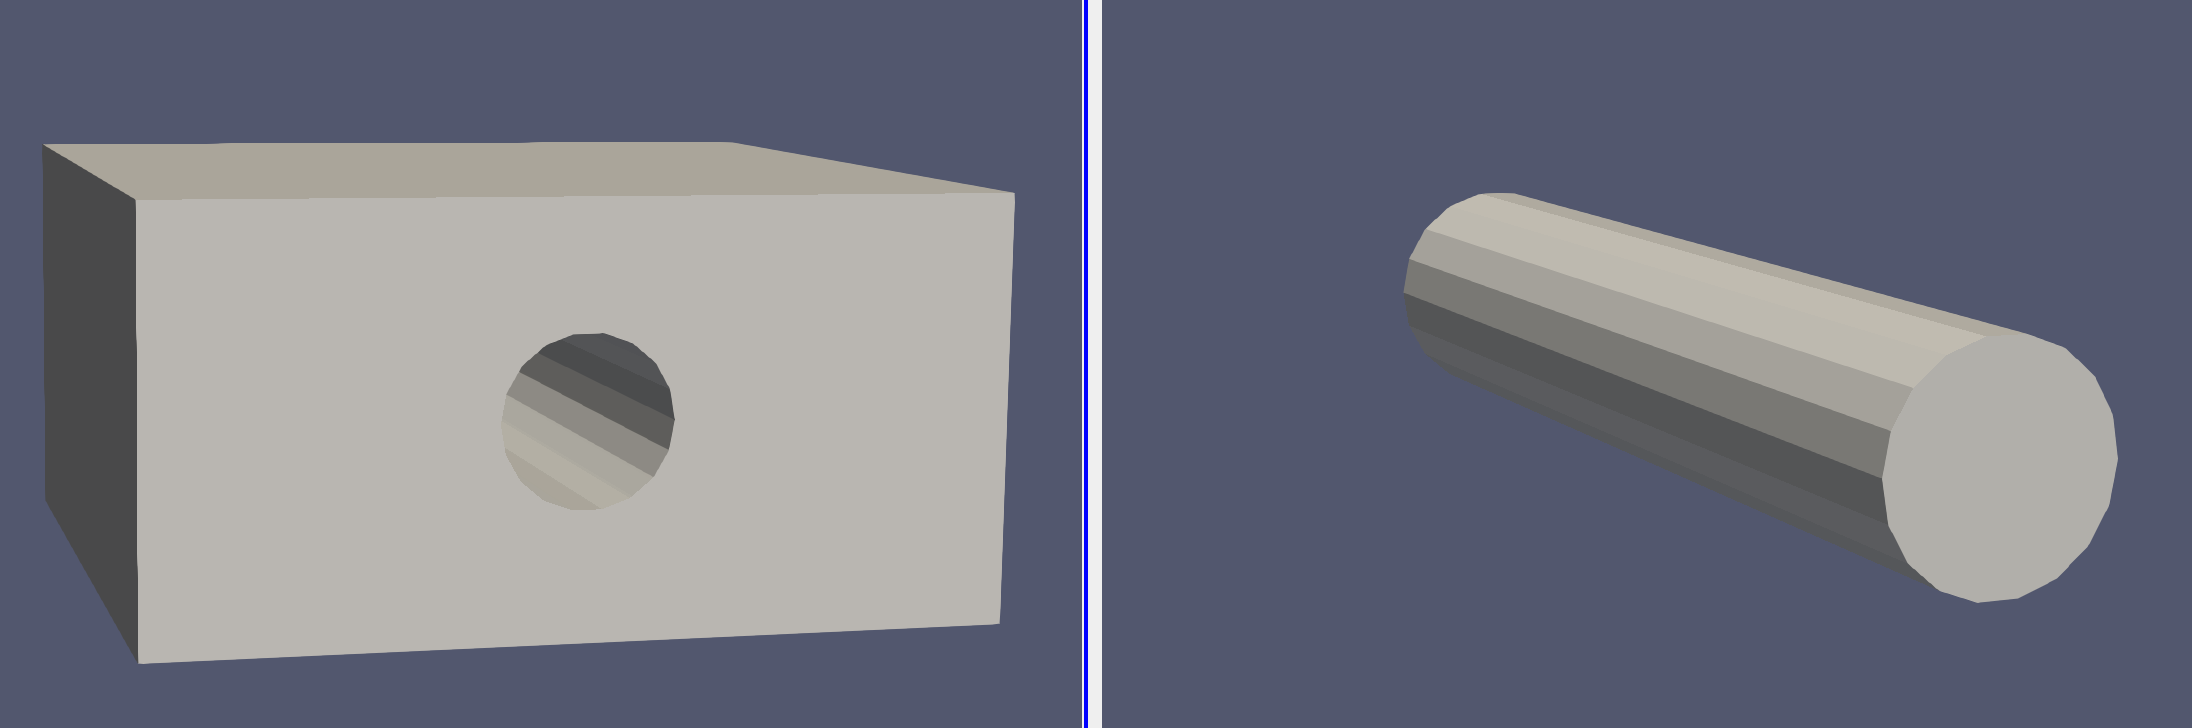
\includegraphics[width=\textwidth]{papers/openfoam/Bilder/vergleich_solution_domain_object.png}
	\caption{Vergleich der Lösungs-Domain (links) und dem 3D-Modell des Objektes (rechts)}
	\label{openfoam:fig:SD_Modell_vergleich}
\end{figure}

In Bild \ref{openfoam:fig:sim_grid} ist zudem ein Beispiel für die Unterteilung der Geometrie in Zellen zu sehen.
Darauf sieht man wie \textbf{snappyHexMesh} das Gitter skaliert.
So besteht in der Umgebung des Objektes das Gitter aus kleinen Zellen und weiter entfernt davon aus grösseren.
Der Grund dafür ist, dass an Orten weiter entfernt von einer Oberfläche die Zellengrösse einen kleineren Einfluss auf die Genauigkeit des Resultates hat.
Man kann so also Rechenaufwand einsparen, indem man nur an Orten kleine Zellen verwendet, an denen der Einfluss der Objekte auf die Flüssigkeit gross ist.
\begin{figure}
	\centering
	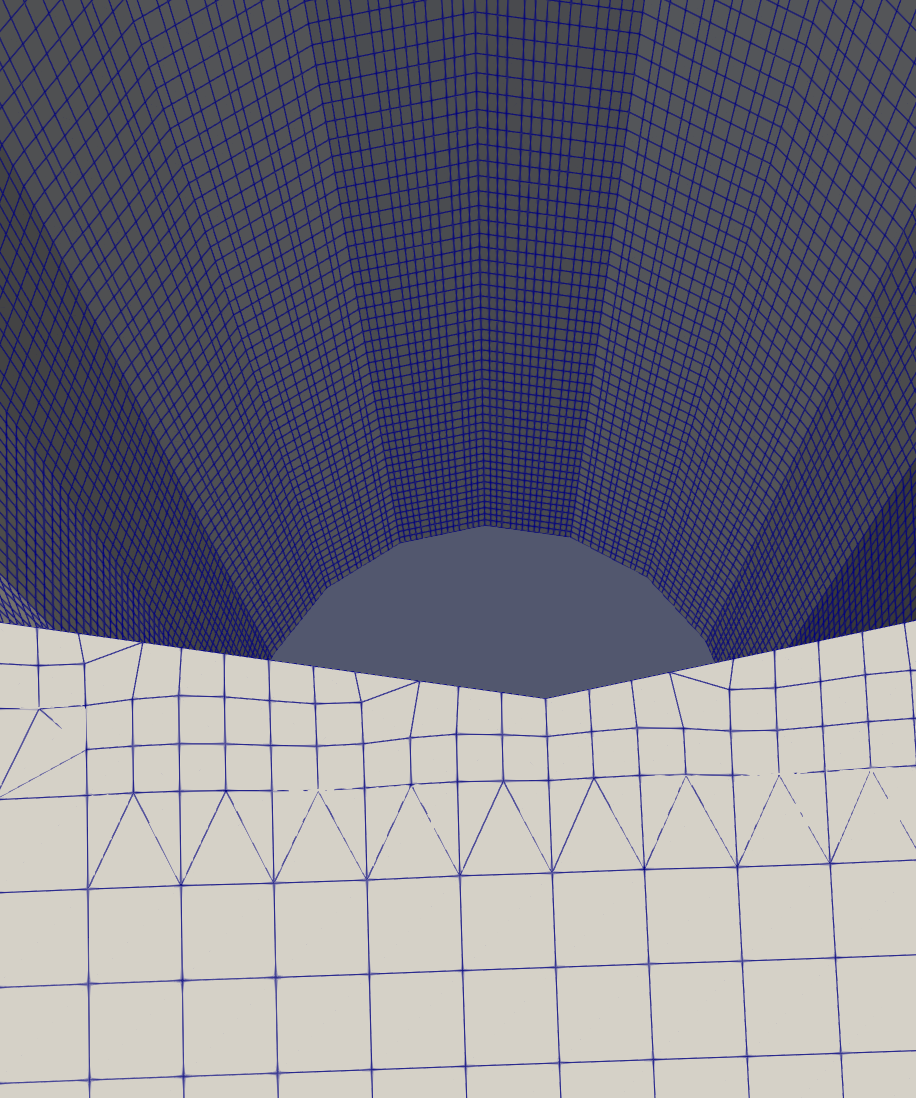
\includegraphics[width=0.5\textwidth]{papers/openfoam/Bilder/grid.png }
	\caption{Beispiel des Rechengitters das von \textbf{snappyHexMesh} generiert wird}
	\label{openfoam:fig:sim_grid}
\end{figure}
Zudem ist auch zu sehen, dass die Zellen nicht unbedingt Würfel sein müssen.
Das Netz kann theoretisch aus beliebigen Polyedern bestehen.
Dies ist aber nicht unbedingt vorteilhaft, denn es ist anzustreben ein Seitenverhältnis der Zellen von ungefähr eins zu wählen. 
Dadurch kann Zeit beim Verarbeiten der 3D-Modelle gespart werden.
Das Vorgehen für diesen Prozess wird in Kapitel \ref{openfoam:section:Mesh erstellen} noch etwas ausführlicher erklärt.
\subsection{Softwarebasiertes Lösen von Differentialgleichungen}
Wenn ein Modell für die Flüssigkeit, die Randbedingungen, das Objekt und dessen Umgebung vorhanden ist, benötigt man nun ein Verfahren, um eine Lösung zu finden. 
Dazu muss die Software als Erstes eine Diskretisierung der Differentialgleichungen, die die Flüssigkeit beschreiben, durchführen.
\index{Diskretisierung}%
Dafür wird das schon diskretisierte Netz der Lösungsdomain genutzt um die komplexen Differentialgleichungen, wie die der Navier-Stokes-Gleichungen, in lineare Gleichungen für jede einzelne der Zellen umzuwandeln.
Um diese Linearisierung zu erreichen, werden jeweils die Eigenschaften der Flüssigkeit, wie Druck, Geschwindigkeit oder Temperatur, am Ort der Zellen durch die Werte in allen benachbarten Zellen berechnet.
So wird der Wert in jeder Zelle, z.B. für Druck $p_{k}$ mit einem Koeffizienten $ a_{i} $ multipliziert und danach mit allen anderen addiert.
Das Resultat ist jeweils ein weiterer Koeffizient $b_{k}$.
Dabei werden die Koeffizienten $a_{k,i}$ und $b_{k }$ jeweils aus den Differentialgleichungen hergeleitet, die Methode dafür unterscheidet sich je nach welcher Methode (FDM, FVM oder FEM).
Dies führt dazu, dass die meisten der Koeffizienten $a_{k,i}$ null sind da die Werte einer Zelle nur von den direkt angrenzenden Zellen abhängig sind.
Diese Summen kann man nun in Matrizenform bringen, dadurch erhält man für jede Eigenschaft eine Gleichung der Form
\begin{equation}
\begin{pmatrix}
	a_{1,1} &  a_{1,2} & a_{1,3} & \dots & a_{1,N} \\
	a_{2,1} &  a_{2,2} & a_{2,3} &  & a_{2,N} \\
	a_{3,1} &  a_{3,2} & a_{3,3} &  & a_{3,N} \\
	\vdots & &  & \ddots & \vdots \\
	a_{N,1} &  a_{N,2} & a_{N,3} & \dots & a_{N,N} \\
\end{pmatrix}
\begin{pmatrix}
	p_{1} \\
	p_{2} \\
	p_{3} \\
	\vdots \\
	p_{N}
\end{pmatrix}
= 
\begin{pmatrix}
b_{1} \\
b_{2} \\
b_{3} \\
\vdots \\
b_{N}
\end{pmatrix}
.
\end{equation}
Um nun den $p$ Vektor zu berechnen wird nicht der Gauss-Algorithmus verwendet, da dies für Matrizen der Grösse, die in CFD Simulationen entstehen, nicht effizient ist.
Stattdessen werden iterative Methoden wie die Gauss-Seidel-Methode verwendet (siehe auch Abschnitt~\ref{buch:pdenumerik:linear:subsection:gauss-seidel}).
Diese führen schon nach wenigen Iterationen zu einer recht genauen Lösung.
